\section{Численные эксперименты}
\subsection{Проверка стабильности имитационной модели}
Для начала проведения численного анализа полученных решений необходимо проверить точность работы реализованной имитационной модели. Для проверки, запустим модель несколько раз с одинаковыми параметрами и для полученных результатов вычислим критерий согласия Колмогорова. Критерий согласия Колмогорова (расстояние Колмогорова) предназначен для проверки гипотезы о том, что некое эмпирическое распределение, в данном случае, распределение, построенное в ходе работы имитационной модели, соответствует предполагаемой модели, которая, в данном случае, так же является результатом работы имитационной модели.

Расстояние Колмогорова вычисляется по следующей формуле
\begin{equation*}
	\Delta_{l} = \underset{0 \leq i \leq \infty}{max}\bigg\rvert \sum_{v=0}^{i} (P(v) - P^{l}(v))\bigg\rvert, l = 1,2
\end{equation*}
Для численного анализа в данной работе применяется система компьютерной алгебры Mathcad. В ней были построены графики распределения вероятностей и вычислено расстояния Колмогорова для двух запусков имитационной модели с одинаковыми параметрами системы

\begin{figure}[H]
	\centering
	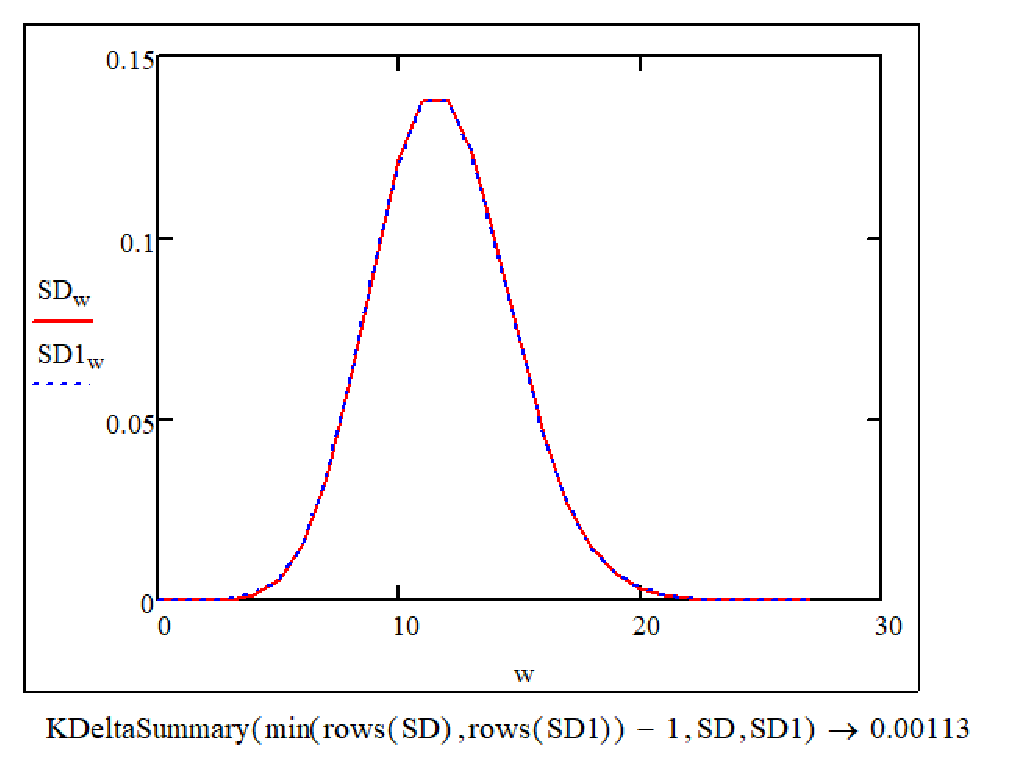
\includegraphics[scale=0.5]{mathcad_check_sim.eps}
	\caption{Сравнение двух отдельных запусков имитационной модели}
	\label{experiments_kol_dist_sim}
\end{figure} 

Как видно на рисунке \ref{experiments_kol_dist_sim}, два отдельных запуска имитационной модели дают практически одинаковые результаты с разницей лишь в 0.00113. На графике распределения полностью накладываются друг на друга. Исходя из этого, можно утверждать, что имитационная модель дает стабильные результаты, следовательно, ее можно использовать для анализа полученных решений и оценки их применимости. 
\subsection{Сравнение распределений вероятностей с эмпирическим распределением}
Теперь, когда стабильность имитационной модели подтверждена экспериментально, сравним результаты работы имитационной модели с полученным асимптотическим приближением функции распределения вероятностей числа обслуженных заявок для систем, рассмотренных в разделах \ref{section_simple_summary}, \ref{section_simple_twodim} и \ref{section_map_twodim} при разной интенсивности возврата заявок с орбиты. Значение этого параметра влияет на точность при сравнении, так как решение систем было получено при асимптотическом условии большой задержки заявок на орбите.



%Таблица точностей
